\documentclass[10pt]{article}
 
\usepackage[margin=1in]{geometry} 
\usepackage{amsmath,amsthm,amssymb, graphicx, multicol, array}
\usepackage{enumitem}
\usepackage{hyperref}
\usepackage[table]{xcolor}
 
\newcommand{\N}{\mathbb{N}}
\newcommand{\Z}{\mathbb{Z}}
 
\newenvironment{problem}[2][]{\begin{trivlist}
\item[\hskip \labelsep {\bfseries #1}\hskip \labelsep {\bfseries #2.}]}{\end{trivlist}}

\date{Due: Oct 30, 2022 10pm PT}

\begin{document}
 
\title{Fall 2022: Midterm Exam}
\author{
CS 181AG: Network Algorithmics}
\maketitle

Under the Honor Code, this document is not to be shared with anyone.

\begin{itemize}

\item The exam will be made available on Gradescope on Tuesday, Oct 25th, 2022 at 8am PT. It will be due Sunday, Oct 30th, 2022 at 10pm PT through Gradescope. Please ensure you leave enough time for the submission process as there is no late allowance for the exam.

\item During the exam, you will have access to your course materials: lecture slides, videos, assignments, textbook, photos of board work from class. You may not access ANY other resources, including other websites, textbooks, or people.

\item Though the exam will be untimed, you will be expected to take it in one sitting. However, you may
take short breaks as needed, e.g. to rest your eyes, grab a snack, change background music, or use the
restroom. Long breaks that include a substantial context switch (e.g. working on another assignment,
having an extended conversation with someone, leaving the area where you’re taking the exam) are
not allowed.

\item You should not contact anyone, including Prof. Arthi, during the exam period. If you have unresolved
questions about the exam, you may include a note about your question and the assumption you made
to address it. Such notes will be taken into consideration when grading the exam.

\item Your exam will be submitted as a PDF. You may answer questions, fill in tables, etc by handwriting, using LaTeX, or any other method you use for your assignments, but you will need to draw for some responses, so prepare to handwrite at least part of the exam. As with all assignments, you will need to mark the answer regions in Gradescope where you put your answers.

\item The exam will be scored out of 100 points over 8 questions, divided by topic

\end{itemize}

\newpage
\textbf{Ethernet.}
\begin{problem}{1: Comparing Media Access Control methods}
\item In class, we learned about several methods for media access control, including Frequency Division Multiple Access (FDMA) and Carrier Sense Multiple Access (CSMA). 

\begin{enumerate}[label=(\alph*)]
 \item Suppose you are designing a local area network for voice calls \emph{only} and that multiple users will want to be on voice calls at the same time (not all on the same call). How well suited is each protocol for this scenario?
 
 FDMA: Since FDMA partitions the different frequencies from which nodes can broadcast within, it follows that since users have their own designated frequencies, multiple conversations could occur at the same time. Thus FDMA would be a suitable choice for this scenario.\\
 
 CSMA: CMSA is not very well suited for this scenario due to the fact that the protocol is reliant on one node transmitting at a time, and thus, only one individual could talk at a time during a phone call. If we wanted to have multiple conversations at the same time,
 this would not fair well as once one person finishes talking, then we would likely have the rest of our individuals attempt to talk at the same time, causing collision issues.\\
 

 \item Suppose you are designing a local area network for sporadic, occasional exchange of large amounts of data between a few users. How well suited is each protocol (FDMA and CSMA) for this scenario?
 
 FDMA: FDMA would not be the suitable choice in this instance due to the fact that we are partitioning our channel bandwidth between our nodes, and thus, even though we do not have all the nodes broadcasting at the same time, not all of the bandwidth is available for nodes to broadcast on. Therefore,
 it will take longer for the large data to be exchanged (due to smaller bandwidth), and thus, exchanges would be far slower than CSMA.\\\\
 
 CSMA: CSMA would be the suitable choice in this instance since we do not have to worry about multiple nodes broadcasting at the same time, and since we can use the full bandwidth when exchanging data which would in-turn mean that the sending of large amounts of data would be faster than with FDMA. Thus, CSMA is well suited for this scenario.\\
 

\end{enumerate}
\end{problem}
\begin{problem}{2: Collision Detection}

Classic Ethernet (802.11) consists of a CSMA/CD network where the time for a signal to get from one end of the wire to the other is 25.6$\mu$s. Consider the scenario where a node \emph{A} transmits a frame at time \textbf{T}. The size of the frame is such that with no collisions, \emph{A} would finish transmitting at \textbf{T + 100$\mu$s}.

\begin{enumerate}[label=(\alph*)]
    \item Is it possible for \emph{A} to detect a collision at time \textbf{T + 45$\mu$s} if no collision was detected between times \textbf{T} and \textbf{T + 45$\mu$s}? Explain why or why not.\\\\
    It is possible for \emph{A} to detect a collision at time \textbf{T + 45$\mu$s}, since it is possible that \emph{A} would not know about a collision until \textbf{T + 51.2$\mu$s} since $d = 25.6$ and \textbf{T + 45$\mu$s} is within that interval. For instance, we could have \emph{A}'s message arrives at the desired node just before the node sends out a message,
    thus meaning that there is a collision that occurs, but that \emph{A} would only find out about at time \textbf{T + 51.2$\mu$s}. 

    \item Is it possible for \emph{A} to detect a collision at time \textbf{T + 60$\mu$s} if no collision was detected between times \textbf{T} and \textbf{T + 60$\mu$s}? Explain why or why not.\\\\
    No, it is not possible for \emph{A} to detect a collision at time \textbf{T + 60$\mu$s} if no collision was detected was detected between times \textbf{T} and \textbf{T + 60$\mu$s}. This is due to the fact that since we did not 
    have a collision within the time period  \textbf{T} and \textbf{T + 51.2$\mu$s}, we can be certain that the desired node knows that \emph{A} is broadcasting which means that it will no longer try to send a message in accordance with CSMA/CD protocol. Thus, the node will wait until it is certain that \emph{A} is done broadcasting before it attempts to broadcast back, meaning that no more collisions will occur, thus no collision can be detected at \textbf{T + 60$\mu$s}.
\end{enumerate}

\end{problem}
\begin{problem}{3: Exponential Backoff}

Upon a collision, remember that each station would like to retransmit as early as possible while lowering the chances of another collision. Your friend suggests the following strategy: upon a collision, pick a random number \emph{x} between 1 and 100 and wait \emph{x} ms before retransmitting. Explain to your friend why exponential backoff is a better approach, given these goals.

\end{problem}
Given our goals of trying to help each station retransmit as early as possible while lowering the chances of another collision, it would make more sense to implement exponential back off instead of a fixed value set to choose the delay time from due to the fact that exponential backoff allows us to scale the amount of time that we want a node to wait before retransmitting a
message based on how congested with think the network is (proxied by the number of collisions a message has had). This scaling helps us minimize the amount of time a message may have to wait if there is a collision, as it gives us the opportunity to send earlier on average than with the choosing random number from 1, 100. The random selection from $\{1,...,100\}$ for the delay time could result in us waiting far longer to retransmit our message for a new slot,
when we may just need to wait a smaller amount of time before retransmitting in comparison with exponential backoff. Similarly, consider that if we had a highly congested network where we have many collisions, exponential backoff would lower the chances of another collision due to the fact that it can increase the size of the set of possible delay times accordingly which would reduce the probability of collisions in the off chance that 
many nodes are trying to send at the same time (such as greater than 100, as this would gaurentee at least two values getting the same length delay), which could happen on a large network. Thus, due to scalability, exponential backoff is the better choice for retransmission strategies.

\newpage
\textbf{Bridging.}
\begin{problem}{4: Bridges and Spanning Tree}
Consider the LAN shown below with 5 bridges (labelled B1 - B5) and 5 nodes (labelled A, C, D, E, and F). 

\begin{figure}[h]
    \centering
    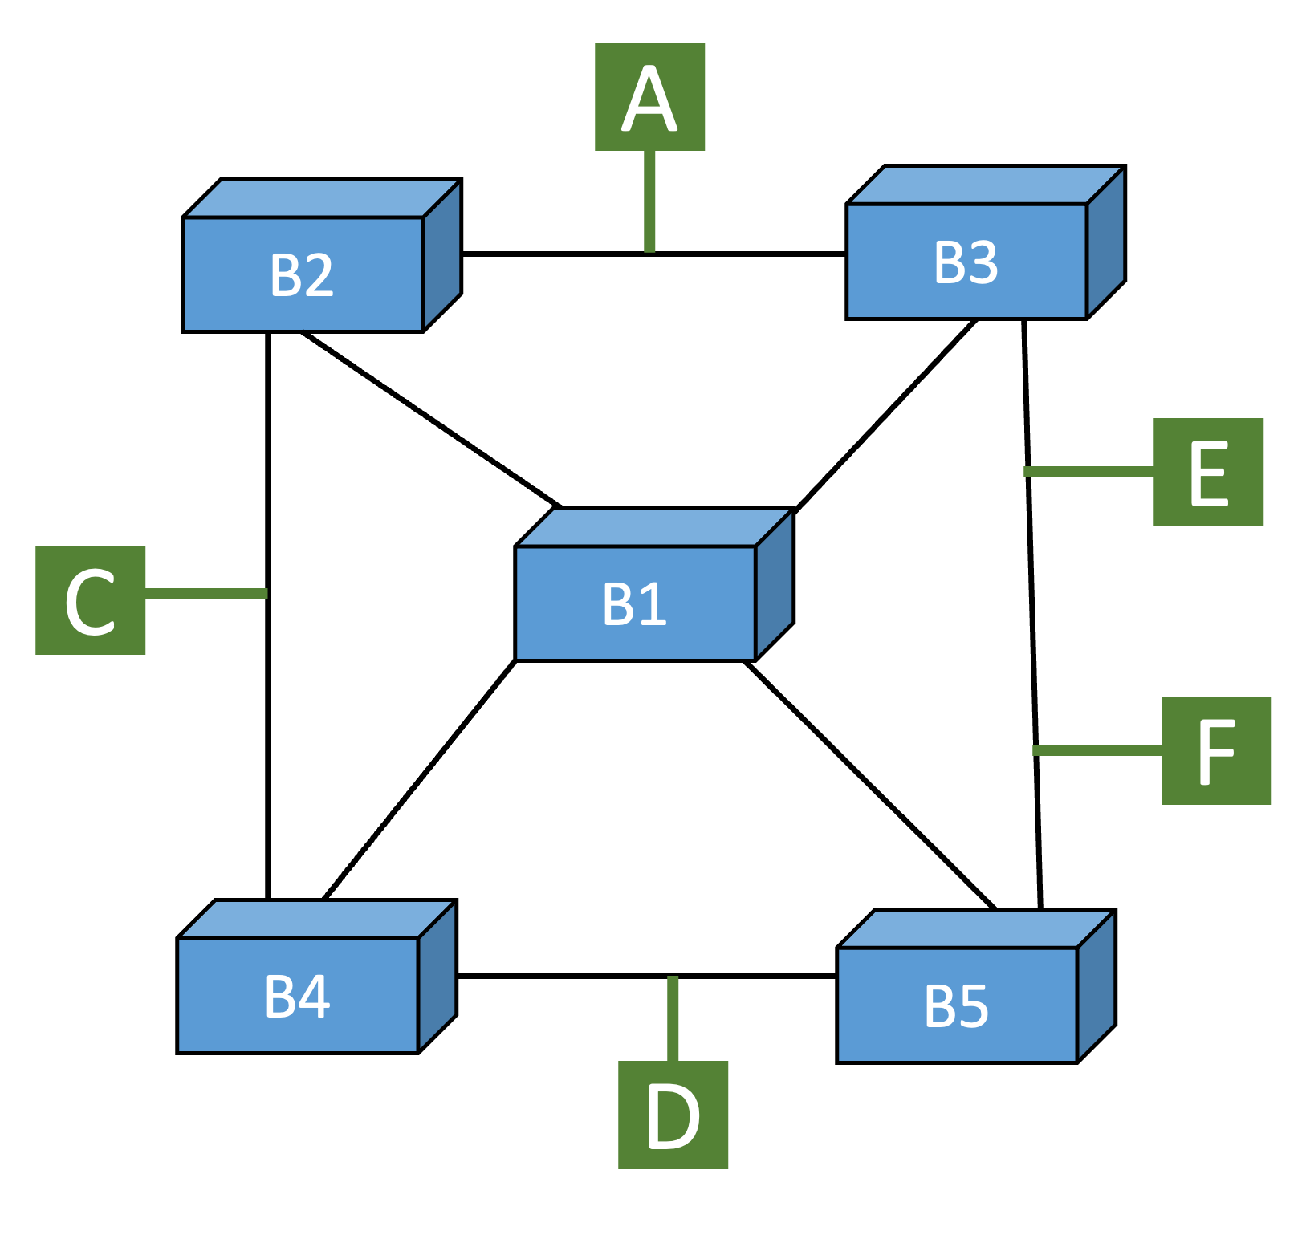
\includegraphics[scale=0.4]{figures/bridges.pdf}
    \label{fig:bin_search}
\end{figure}


\begin{enumerate}[label=(\alph*)]
    \item After the spanning tree protocol is run, which ports will be turned off? You can either describe them (e.g., ``Bx's port that faces By'') or clearly draw an ``x'' over the port in the image. \\\\
    The ports that will be turned off after the spanning tree protocol is run will be B4's port that faces B2, B5's port that faces B4, B5's port that faces B3, and B3's port that faces B2.
    \item  \textbf{Assume that the spanning tree protocol has now run, the ports you marked are now turned off, and all bridges have empty learning tables}. When node A sends a message to node E, 
    
    1) Which bridges learn about A's location? \\\\
    When node A sends a message to node E, the bridges that learns about A's location are B1, B2, B3, B4, and B5, due to the fact that since all learning tables are empty, no bridge knows where A is, so it subsequently forwards the message to all of its branches.

    2) Which other nodes hear A's message, whether it was intended for them or not? \\\\
    All other nodes will hear A's message.
    \item \textbf{After part b}, when node E sends a message to node A, 
    
    1) Which bridges learn about E's location? \\\\
    Bridges B3, B1, and B2 will learn about E's location since they know which port A is at and thus, can forwards the message onto the correct port.

    2) Which other nodes hear E's message, whether it was intended for them or not?\\\\
    The nodes F and A will hear E's message.
    \item \textbf{After part c}, when node D sends a message to node E, 
    
    1) Which bridges learn about D's location? \\\\
    Bridges B4, B1, and B3 will learn about D's location, since B1 and B3 know which port E is at and can subsequently forwards to the correct port.

    2) Which other nodes hear D's message, whether it was intended for them or not? \\\\
    Only E and F hear D's message.
\end{enumerate}
\end{problem}
\newpage
\textbf{Routing Protocols}
\begin{problem}{5: Distance-Vector}
Suppose we have the following routers, x, y and z, that run a distance-vector protocol to exchange shortest path information.
\begin{figure}[h]
    \centering
    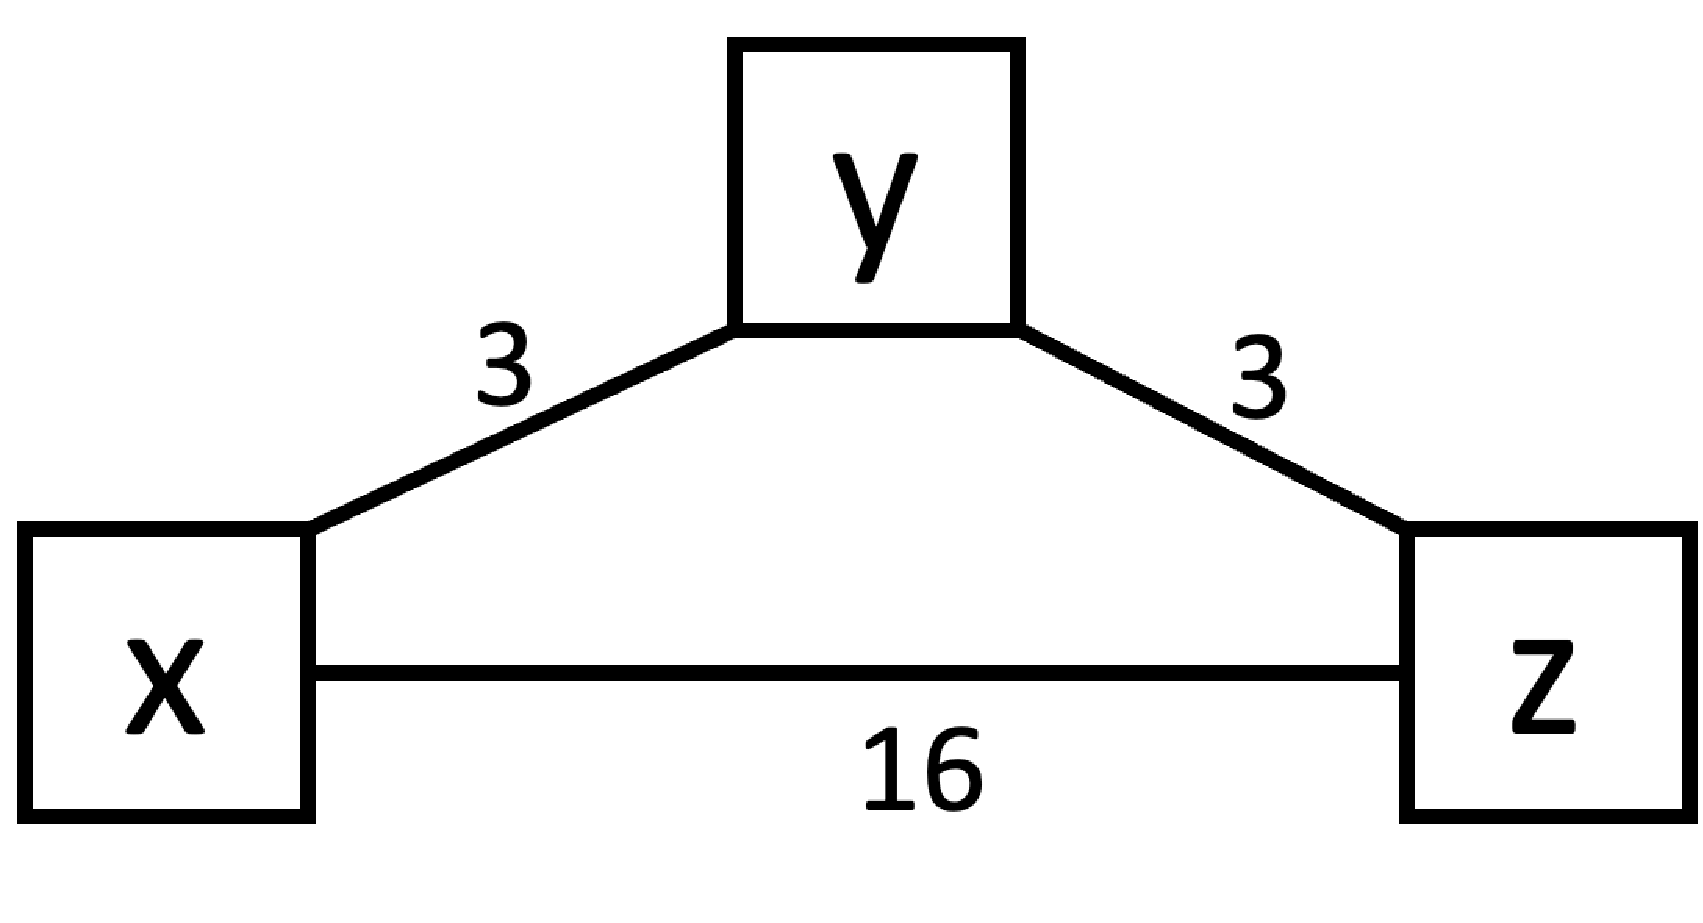
\includegraphics[scale=0.3]{figures/dv_routing.pdf}
    \label{fig:bin_search}
\end{figure}
\begin{enumerate}[label=(\alph*)]
    \item Fill in each router's table of shortest paths \textbf{after} the protocol has converged. \\
    
\begin{tabular}{|c|c|c|}
\hline
\multicolumn{3}{|c|}{\textbf{x's table}}\\
\cline{1-3}
Node & Distance & Next Hop\\
\hline
y & 3 & y \\
\hline
z & 6 & y\\
\hline
\end{tabular}

\begin{tabular}{|c|c|c|}
\hline
\multicolumn{3}{|c|}{\textbf{y's table}}\\
\cline{1-3}
Node & Distance & Next Hop\\
\hline
x & 3 &x \\
\hline
z & 3&z \\
\hline
\end{tabular}

\begin{tabular}{|c|c|c|}
\hline
\multicolumn{3}{|c|}{\textbf{z's table}}\\
\cline{1-3}
Node & Distance & Next Hop\\
\hline
x & 6 & y\\
\hline
y & 3& y\\
\hline
\end{tabular}
    \item After the protocol has converged (i.e., it is in a steady state), the link between x and y breaks. Before y can tell z anything, y receives a message from z advertising its route to x. Fill in the table below to reflect the contents of z's message and the next 5 messages between y and z regarding their distance to x. Assume poison reverse is not used. Please ignore the shaded cells and only fill in the ones marked ``Distance to x: ''.  
    
\begin{table}[ht]
\begin{center}
\begin{tabular}{|p{4cm}|p{4cm}|}
	\hline
	\textbf{y} & \textbf{z}\\
	\hline
	\cellcolor{gray!50} & Distance to x: 6   \\
	\hline
	Distance to x: 9  & \cellcolor{gray!50}\\
	\hline
	\cellcolor{gray!50} & Distance to x: 12   \\
	\hline
	Distance to x: 15   & \cellcolor{gray!50}\\
	\hline
	\cellcolor{gray!50} & Distance to x: 16   \\
	\hline
	Distance to x:  19  & \cellcolor{gray!50}\\
	\hline
	
\end{tabular}
\end{center}
\end{table}
\end{enumerate}
\end{problem}
\newpage
\textbf{Longest Matching Prefix}
\begin{problem}{6: Comparing LPM methods}
In class, we learned about several ways of representing IP prefixes for lookup, including 1) the unibit trie, 2) the multibit trie, and 3) the Lulea compressed trie. 
\begin{enumerate}[label=(\alph*)]
    \item If our goals were fast lookup and fast insertion and we did \emph{not} care about memory, which of the three methods listed above is the best fit? \\\\
    If we wanted fast lookup and fast insertion and did not care about memory, the best method listed above is a multibit trie.
    \item If our goals were low memory usage and fast insertion and we did \emph{not} care about lookup time, which of the three methods listed above is the best fit? \\\\
    If we wanted low memory usage and fast insertion but that we do not care about lookup time, we would wante to use a Lulea compressed trie.
    \item If our goals were low memory usage and fast lookup time and we did \emph{not} care about insertion time, which of the three methods listed above is the best fit? \\\\
    If our goals were low memory usage and fast lookup time but poor insertion time, the unibit trie would be our best choice.
\end{enumerate}
\end{problem}
\newpage
\begin{problem}{7: Binary Search on Prefix Lengths}
Consider the use of binary search on prefix lengths, as described in class, where we keep an array of tables, each containing prefixes of a different length, sorted by prefix length. Similar to the example from class, we add markers to direct the search towards the right half. When a table is searched, the three possible results are 1) a matching prefix was found 2) a matching marker was found 3) neither a matching prefix nor a matching marker were found. \textbf{However, suppose we only added markers and did \emph{not} store the best matching prefix along with the marker.} Then, the algorithm must backtrack and \emph{also} search the left half of the array if a matching prefix is not found in either the middle table or on the right half. The algorithm pseudocode is as follows. 

\begin{verbatim}
    search(IP, array):
        if length of array is 0:
            return None
        mid = result of checking IP against middle table
        if mid = matching prefix found:
            save prefix as best match so far
        if mid = (matching prefix found OR matching marker found):
            right = search(IP, right half of array)
            if right exists: # Valid prefix was found in right half
                return right
            else if there exists a best match so far:
                return best match so far
            else:
                return search(IP, left half of array)
        else: # Neither a matching prefix nor matching marker was found in the middle table
            return search(IP, left half of array)
\end{verbatim}
Your friend tells you that the backtracking algorithm can't be that bad because it doesn't add many searches. However, you show that the backtracking algorithm can in fact lead to checking every single table, or a O(n) search in the worst case. 
\\Make your point using the array of tables below (with prefix lengths ranging from 1 to 7) and the IP address \textbf{11001101} (for simplicity, let's use IP addresses that are only 8 bits long). Your job is to fill in prefixes and corresponding markers that would lead to this algorithm checking every table in the array. Please clearly distinguish markers from prefixes by adding ``M:'' or ``P:'' before each entry in the table.
    
Hints: In what order would the search need to check tables for it to hit every table? What markers must exist such that this order is followed? Finally, what prefixes must exist for these markers to have been inserted? There are multiple correct responses - anything that searches each table is valid.

\begin{table}[ht]
\begin{center}
\begin{tabular}{|p{2cm}|p{2cm}|p{2cm}|p{2cm}|p{2cm}|p{2cm}|p{2cm}|}
	\hline
	\textbf{Prefix Length = 1} & \textbf{Prefix Length = 2} & \textbf{Prefix Length = 3}& \textbf{Prefix Length = 4}& \textbf{Prefix Length = 5}& \textbf{Prefix Length = 6}&\textbf{Prefix Length = 7}\\
	\hline
    P: 1* & P: 10*, M: 11* & & P: 1101*, M: 1100* & & P: 111111*, M: 110011* &\\[40pt]
	\hline
	
\end{tabular}
\end{center}
\end{table}
\end{problem}
\newpage
\textbf{Packet Classification}
\begin{problem}{8: Grid of Tries}
In class we learned about three methods when using a grid of tries to find the least-cost rule that matches destination and source IP addresses: 1) form the grid of tries, adding each source prefix exactly once, and use a backtracking algorithm to find the best matching rule 2) form the grid of tries, adding each source prefix to \emph{every} source trie corresponding to a matching destination prefix and do \emph{not} backtrack, and 3) form the grid of tries, adding each source prefix exactly once, and use switch pointers to move between the different source tries.

\begin{enumerate}[label=(\alph*)]
    \item For the rules shown in the table below, draw the third method. Show the grid of tries and the switch pointers. Please distinguish clearly between source and destination tries (different colors or dashed lines between them).
    \begin{table}[ht]
    \begin{center}
    \begin{tabular}{|c|c|c|}
    	\hline
    	 & Destination & Source\\
    	\hline
    	R1 & 00* & 10* \\
    	\hline
    	R2 & 0* & 11*\\
    	\hline
    	R3 & 00* & 1*\\
    	\hline
    	R4 & 0* & 0*\\
    	\hline
    	R5 & * & 01*\\
    	\hline
    	R6 & * & *\\
    	\hline
    	
    \end{tabular}
    \end{center}
    \end{table}
\begin{center}
    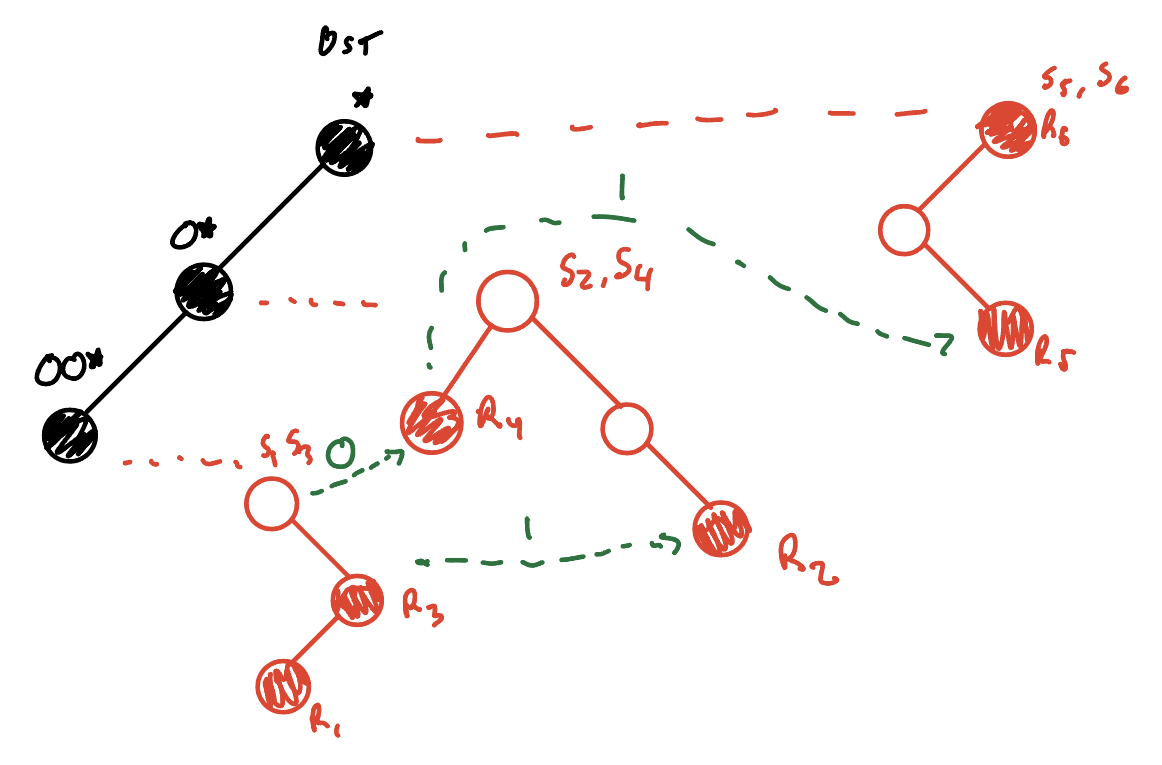
\includegraphics[scale = 0.35]{IMG_8C8A29BBB830-1.jpeg}
\end{center}

\item What is the main advantage of method 3 over method 1?\\\\
The main advantage of method 3 over method 1 is the fact that we no longer have to backtrack back through our trie, which makes rule lookup significantly faster.
\item What is the main advantage of method 3 over method 2?\\\\
The main advantage of method 3 over method 2 is the fact that we do not have to store the complete source trie of valid prefixes for each of our tries. Thus, the use of pointer switches allows us to reduce the amount of memory that our structure takes up.
\end{enumerate}


\end{problem}
\newpage
\begin{problem}{9}
How long did this midterm take you? How would you rate the difficulty on a scale from 1-10 (10 being the hardest)? Feel free to share any other thoughts on the midterm or your preparation.
\end{problem}
This midterm took me $\approx 3.\overline{3}$ hours. I would rate the difficulty as varied based on problem, but generally around a 7.
\end{document}

